\documentclass[a4paper,12pt]{article}
\usepackage[utf8]{inputenc}
\usepackage[T1]{fontenc}
\usepackage{graphicx} % Pour insérer des images
\usepackage{hyperref} % Pour insérer des liens cliquables
\usepackage{geometry} % Pour ajuster les marges
\usepackage{float} % Pour forcer le placement des figures
\usepackage{xcolor} % Pour les couleurs
\usepackage{lipsum} % Pour générer du texte d'exemple

\geometry{margin=2.5cm} % Marges de 2.5 cm

% Définition de couleurs personnalisées
\definecolor{myblue}{RGB}{0, 102, 204}
\definecolor{mygreen}{RGB}{34, 153, 84}
\definecolor{myorange}{RGB}{255, 140, 0}
\definecolor{mypurple}{RGB}{153, 51, 204}

\begin{document}

% Titre principal avec couleur
\begin{titlepage}
    \centering
    {\LARGE \textbf{\color{myblue} Mon Projet personnel et professionnel}} \\[1cm]
    {\Large Organisation d'Événements : \textbf{\color{mypurple} Prestige Event}} \\[2cm]
    \vfill
    {\large Préparé par : Khadija Ben Majdoub groupe 4} \\[0.5cm]
    {\large Décembre 2024}
    \vfill
\end{titlepage}

% Introduction
\section*{\color{myblue} Introduction}
Ce rapport présente les travaux réalisés dans le cadre du module de Projet Personnel et Professionnel (PPP). Au cours de ce module, nous avons travaillé sur cinq ateliers pour développer nos compétences personnelles et professionnelles.  

Les sections suivantes regroupent les livrables réalisés pendant le module, notamment mon CV, ma lettre de motivation, mon analyse SWOT, et des visualisations statistiques pertinentes.

% Section 1 : Mon CV
\section*{\color{mygreen} Atelier 1 : Mon CV}
Voici une copie de mon CV :  

\begin{figure}[H]
    \centering
    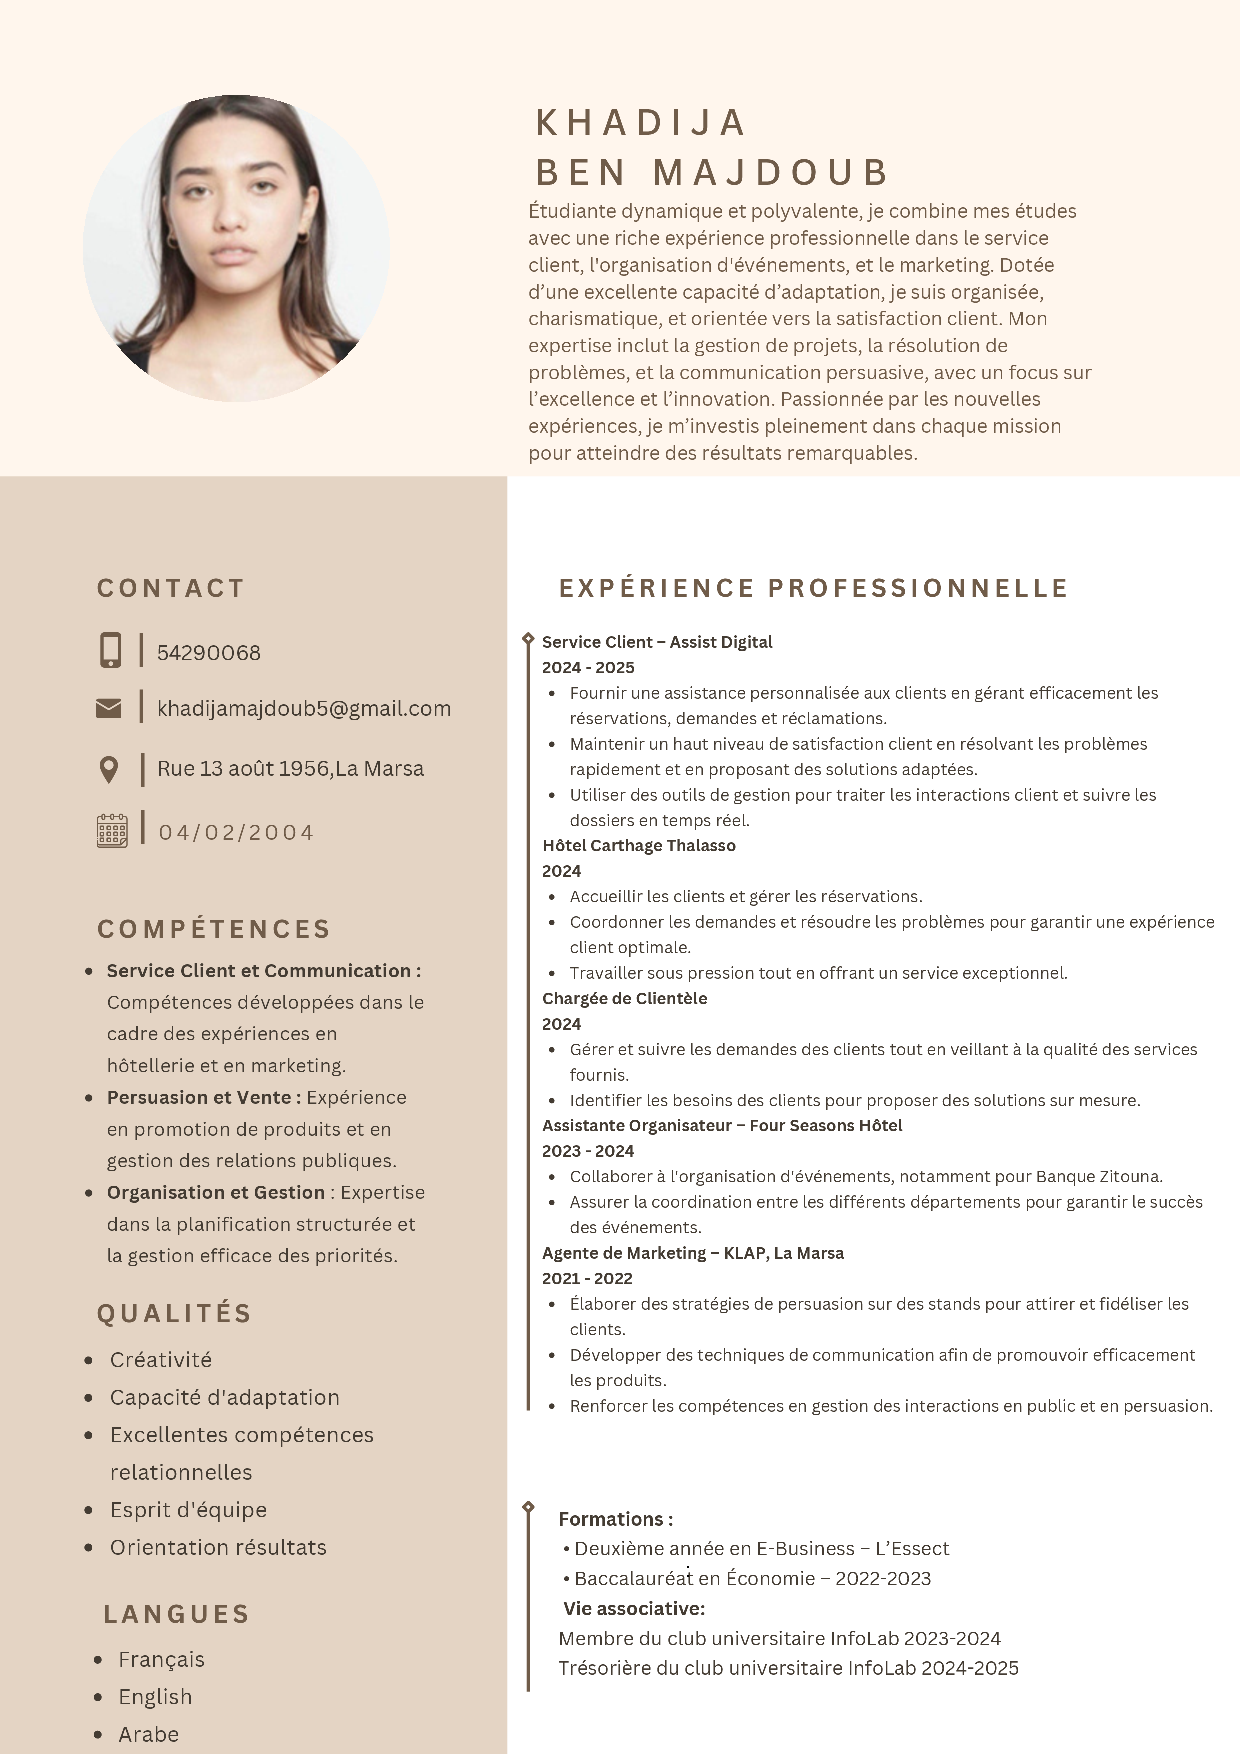
\includegraphics[width=\textwidth]{CV.pdf} % Remplace "cvimage.png" par le nom de ton fichier CV
    \caption{Mon CV}
    \label{fig:cv}
\end{figure}

% Section 2 : Lettre de motivation
\section*{\color{mygreen} Atelier 2 : Lettre de Motivation}
Voici une copie de ma lettre de motivation :  

\begin{figure}[H]
    \centering
    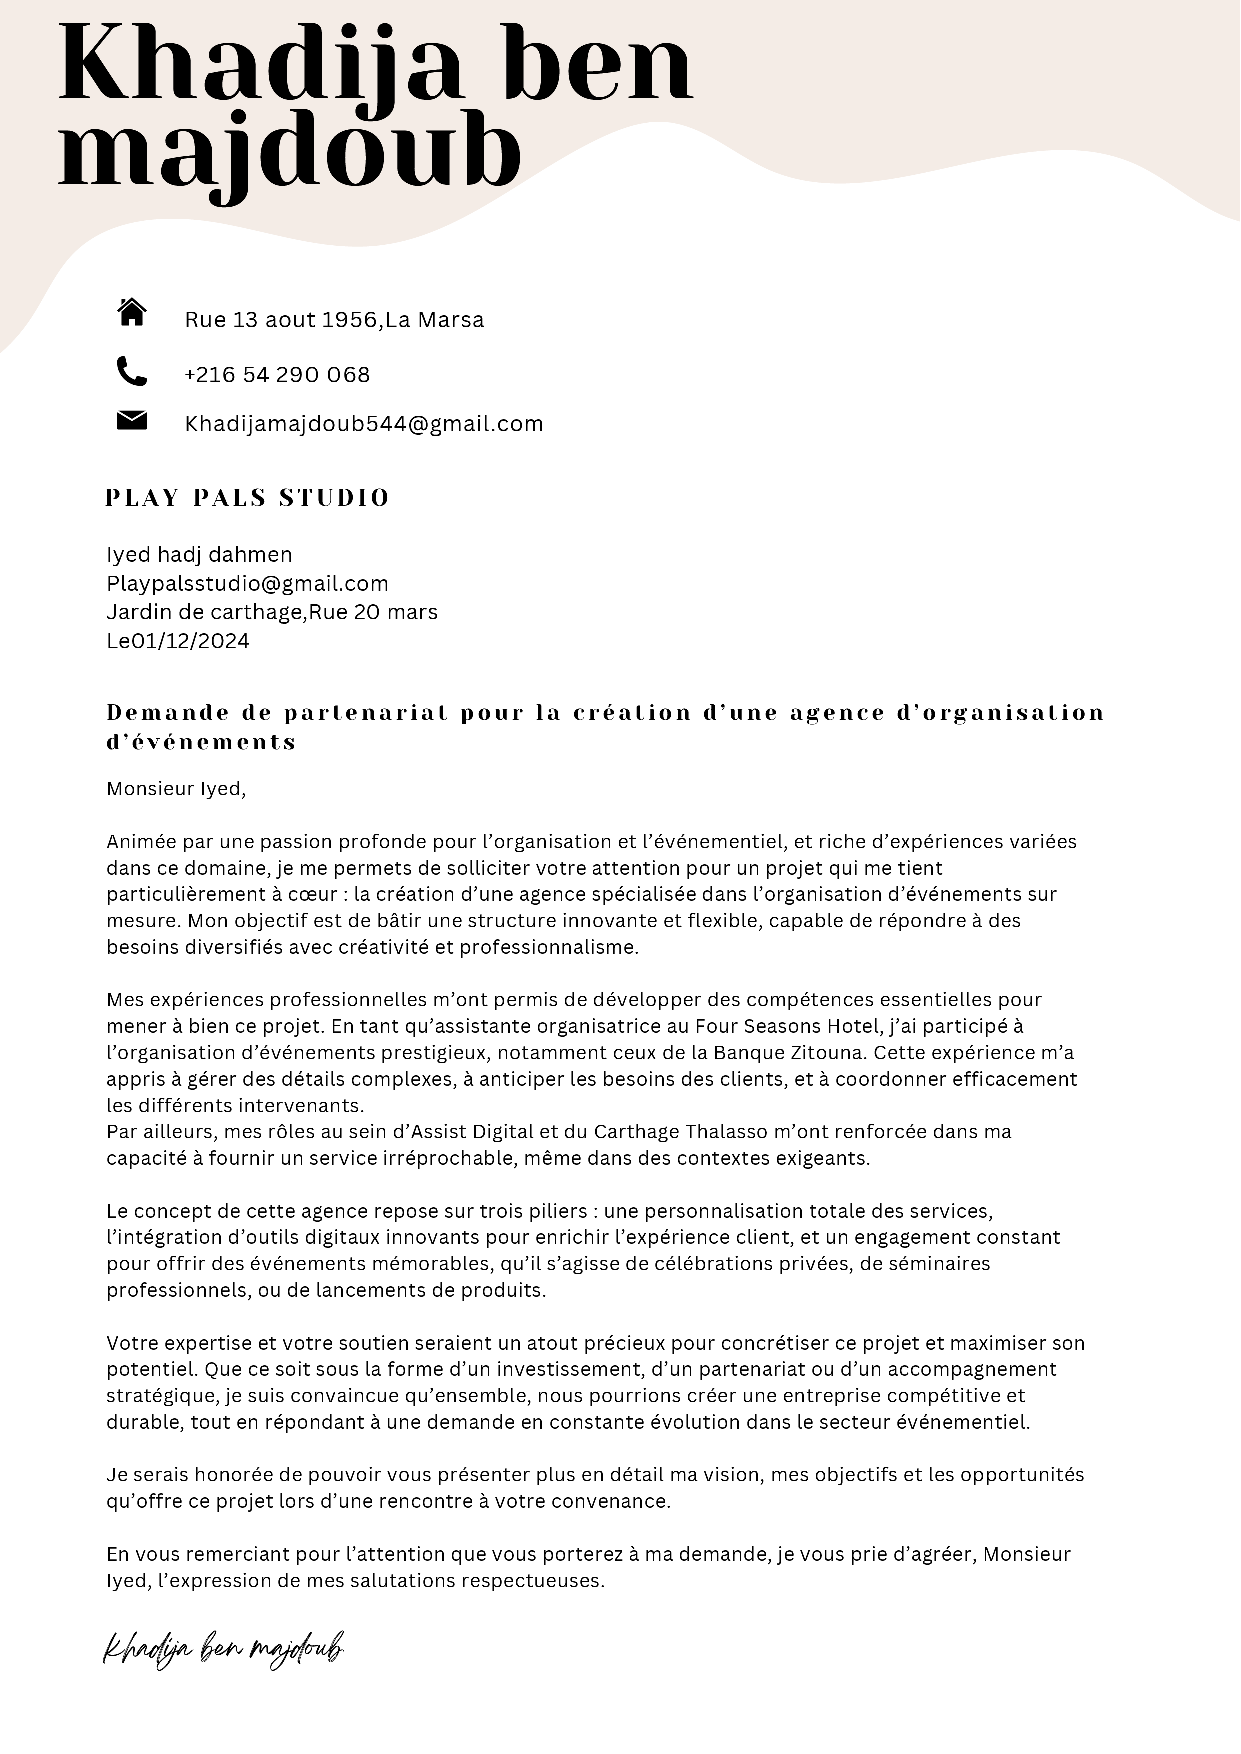
\includegraphics[width=\textwidth]{lettredemotivation.pdf} % Remplace "lettremotivation.png" par le nom de ton fichier
    \caption{Ma lettre de motivation}
    \label{fig:lettre}
\end{figure}

% Section 3 : Réseautage - LinkedIn
\section*{\color{mygreen} Atelier 3 : Réseautage - LinkedIn}
Pour élargir mon réseau professionnel, j'ai optimisé mon profil LinkedIn. Vous pouvez le consulter en suivant le lien ci-dessous : 
https://www.linkedin.com/in/khadija-ben-majdoub-a42a902a0/

\bigskip
\href{https://www.linkedin.com/in/khadija-ben-majdoub-a42a902a0}{\textbf{\color{myorange} Mon Profil LinkedIn}}

% Section 4 : Le choix de mon projet professionnel - Analyse SWOT
\section*{\color{mygreen} Atelier 4 : Le Choix de Mon Projet Professionnel}
Voici une analyse SWOT réalisée pour mon projet d'entreprise, Prestige Event :  

\bigskip
\textbf{\color{myblue} Forces (Strengths)} :  
- Expertise et créativité.  
- Compétences organisationnelles solides.  
- Adaptabilité aux différents types d'événements.  
- Réseau de prestataires locaux.  
- Passion pour l'excellence.  

\bigskip
\textbf{\color{myblue} Faiblesses (Weaknesses)} :  
- Ressources initiales limitées.  
- Faible visibilité au lancement.  
- Dépendance à des tiers.  
- Manque d'expérience spécifique.  

\bigskip
\textbf{\color{myblue} Opportunités (Opportunities)} :  
- Demande croissante pour des événements personnalisés.  
- Intégration des technologies numériques.  
- Popularité des événements écoresponsables.  
- Expansion vers des marchés internationaux.  

\bigskip
\textbf{\color{myblue} Menaces (Threats)} :  
- Concurrence intense.  
- Vulnérabilité à l'économie.  
- Risques sanitaires.  
- Activité saisonnière.  

% Section 5 : Découverte du PPP
\section*{\color{mygreen} Atelier 5 : Découverte du PPP}
Cet atelier m'a permis de découvrir l'importance des outils statistiques dans la gestion de projets. Voici cinq graphiques représentatifs des données collectées pour mon entreprise d'organisation d'événements :  

\begin{figure}[H]
    \centering
    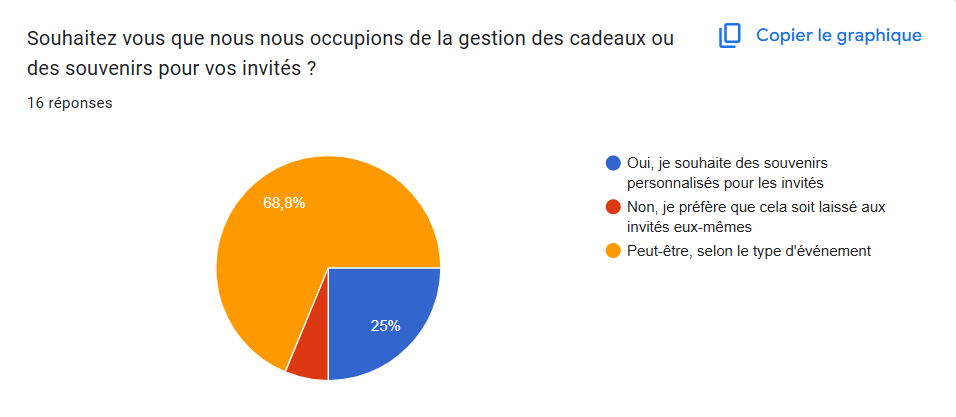
\includegraphics[width=0.6\textwidth]{stat1.png} % Remplace par tes fichiers image
    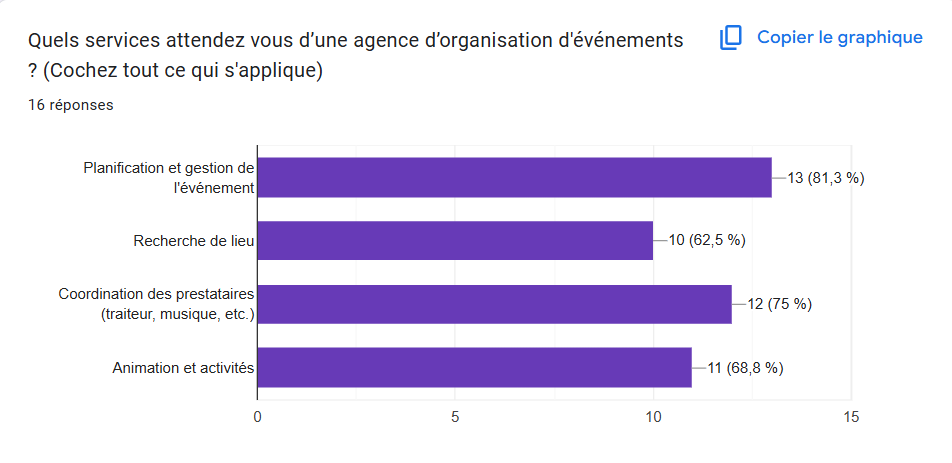
\includegraphics[width=0.6\textwidth]{stat2.png}
    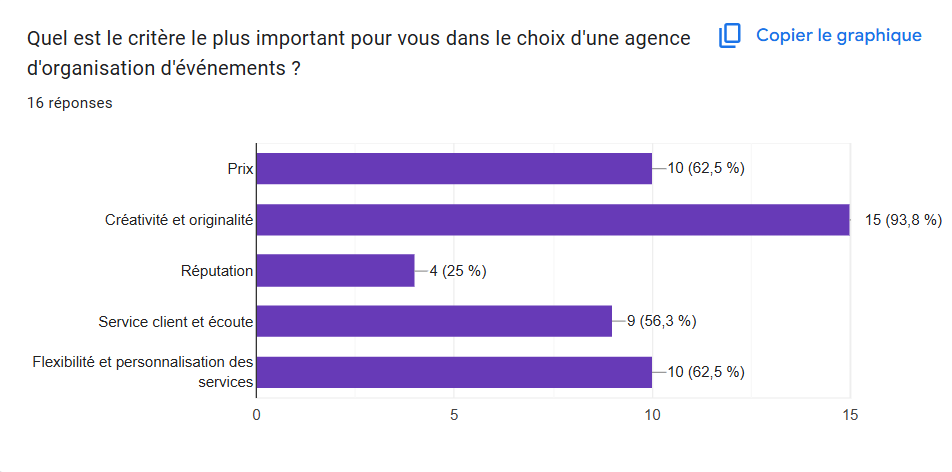
\includegraphics[width=0.6\textwidth]{stat3.png} \\[0.5cm]
    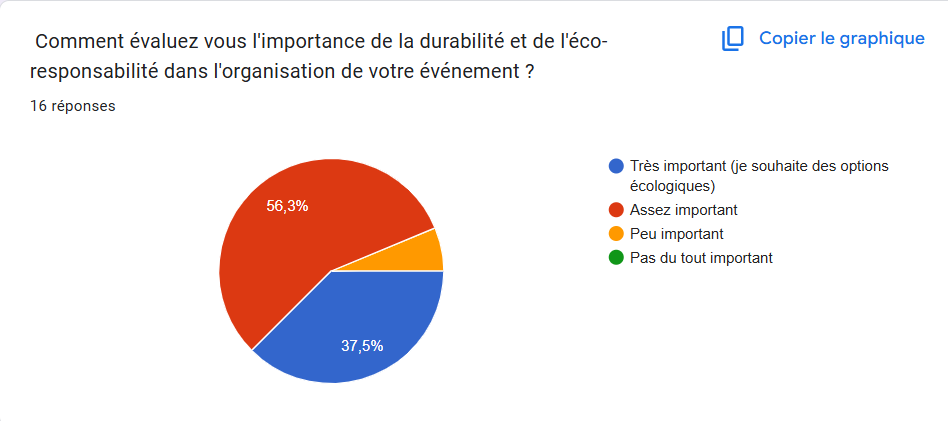
\includegraphics[width=0.6\textwidth]{stat4.png}
    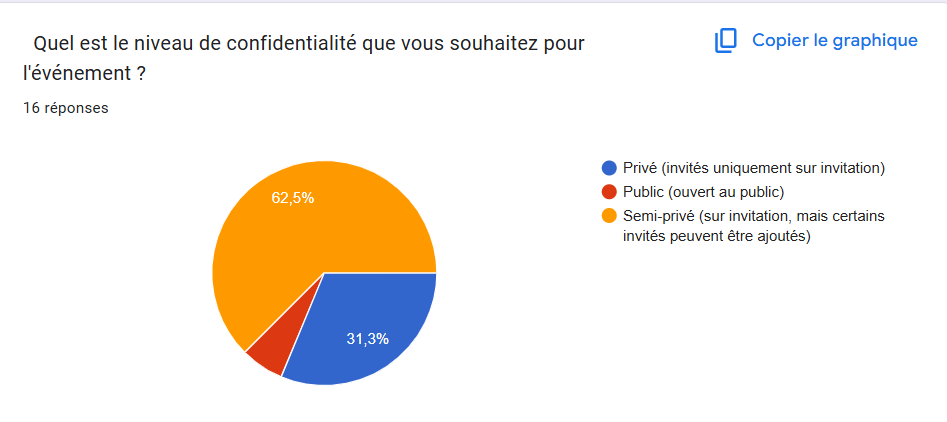
\includegraphics[width=0.6\textwidth]{stat5.png}
    \caption{Statistiques recueillies pour Prestige Event}
    \label{fig:stats}
\end{figure}

% Section 6 : Questionnaire
\section*{\color{myblue} Questionnaire}
Dans le cadre de ce projet, j'ai publié un questionnaire pour recueillir des informations utiles sur le marché de l'organisation d'événements. Ce questionnaire m'a aidé à mieux comprendre les attentes et besoins de mes futurs clients potentiels.  

\bigskip
En résumé:

Les personnes interrogées sont généralement très impliquées dans l'organisation de leurs événements, notamment en ce qui concerne la gestion de cadres ou de souvenirs. Elles attendent principalement des agences d'organisation d'événements qu'elles s'occupent de la planification, de la logistique et de la gestion des invités. Le choix d'une agence se fait principalement en fonction de sa crédibilité, de son expérience et du prix proposé. La durabilité et la responsabilité sont des critères de plus en plus importants dans l'organisation d'événements. Enfin, la confidentialité est une préoccupation majeure pour la majorité des personnes interrogées.

% Conclusion
\section*{\color{myblue} Conclusion}
En conclusion, ce projet de PPP m’a permis de faire un point précis sur mes compétences, mes expériences et mes objectifs professionnels. À travers les différents ateliers et livrables réalisés, j’ai pu identifier mes points forts et mes axes d’amélioration, ce qui m’a permis de mieux orienter mon projet professionnel. 

L’analyse SWOT de mon projet d’organisation d’événements, ainsi que les réflexions sur mes qualités et défauts, m’ont offert une vision plus claire de mes aspirations et des défis auxquels je serai confrontée. Ce travail m’a également permis de mieux comprendre les réalités du secteur de l’événementiel et de me projeter dans un avenir professionnel passionnant. 

Je suis désormais plus confiante et déterminée à poursuivre ma carrière dans ce domaine, en continuant à développer mes compétences et à m’adapter aux évolutions du marché. Mon projet est en constante évolution, et je suis convaincue qu’il me permettra de m’épanouir tout en contribuant au succès des événements que je gérerai.

\end{document}
